\documentclass[aspectratio=169,11pt]{beamer}
\usetheme{Madrid}
\usecolortheme{default}
\setbeamertemplate{navigation symbols}{}
\setbeamertemplate{items}[circle]
\setbeamercovered{transparent}
\usepackage[utf8]{inputenc}
\usepackage[T1]{fontenc}
\usepackage{lmodern}
\usepackage{amsmath,amssymb}
\usepackage{graphicx}
\usepackage{booktabs}
\usepackage{array}
\usepackage{ragged2e}
\usepackage{tikz}
\usepackage{tcolorbox}
\usepackage{multicol}
\usetikzlibrary{positioning,calc,shapes.geometric,arrows.meta}

\definecolor{UNBCGreen}{RGB}{0,102,51}
\definecolor{UNBCDark}{RGB}{0,74,37}
\definecolor{UNBCGold}{RGB}{189,155,96}
\definecolor{SoftCream}{RGB}{249,247,242}
\definecolor{SoftGray}{RGB}{244,246,248}
\definecolor{AccentBlue}{RGB}{41,98,255}
\definecolor{AccentOrange}{RGB}{230,126,34}
\definecolor{AccentTeal}{RGB}{0,150,136}
\definecolor{AccentRed}{RGB}{192,57,43}

\setbeamercolor{normal text}{fg=black,bg=white}
\setbeamercolor{structure}{fg=UNBCGreen}
\setbeamercolor{title}{fg=white,bg=UNBCGreen}
\setbeamercolor{subtitle}{fg=UNBCGold}
\setbeamercolor{frametitle}{fg=white,bg=UNBCGreen}
\setbeamercolor{block title}{fg=white,bg=UNBCGreen}
\setbeamercolor{block body}{fg=black,bg=SoftGray}
\setbeamercolor{item}{fg=UNBCGreen}
\setbeamercolor{section in toc}{fg=UNBCGreen}
\setbeamertemplate{headline}{}
\setbeamertemplate{footline}{%
  \leavevmode%
  \hbox{%
  \begin{beamercolorbox}[wd=.78\paperwidth,ht=2.8ex,dp=1.2ex,leftskip=1em]{author in head/foot}%
  \color{UNBCDark}\textbf{UNBC Economics} \hspace{0.5em} \textcolor{UNBCGold}{|} \hspace{0.5em} Economics Is Everywhere
  \end{beamercolorbox}%
  \begin{beamercolorbox}[wd=.22\paperwidth,ht=2.8ex,dp=1.2ex,rightskip=1em plus1fil]{date in head/foot}%
  \color{UNBCDark}\insertframenumber/\inserttotalframenumber
  \end{beamercolorbox}}%
}

\newtcolorbox{mybox}[2][]{
  colback=#2!8,
  colframe=#2,
  boxrule=0.8pt,
  arc=2mm,
  left=2mm,right=2mm,top=1.5mm,bottom=1.5mm,
  #1
}

\newcommand{\topbanner}[1]{%
\begin{tikzpicture}[remember picture,overlay]
\fill[UNBCGold] ([yshift=-0.65cm]current page.north west) rectangle ([yshift=-0.48cm]current page.north east);
\node[anchor=north west,font=\small\bfseries,text=UNBCDark] at ([xshift=0.35cm,yshift=-0.78cm]current page.north west) {#1};
\end{tikzpicture}%
}

\title{Economics Is Everywhere}
\subtitle{A visual 20-minute introduction for students and parents}
\author{UNBC-branded presentation}
\date{}

\begin{document}

% Title slide
{
\usebackgroundtemplate{\includegraphics[width=\paperwidth,height=\paperheight]{/mnt/data/user-fE7TD4iShS4hrCs2AD7Tw51y/5c309b8515dc4e28a392dd530e83cc2b/mnt/data/econ_montage.png}}
\begin{frame}[plain]
\begin{tikzpicture}[remember picture,overlay]
\fill[UNBCDark,opacity=0.80] (current page.south west) rectangle (current page.north east);
\fill[UNBCGold,opacity=0.95] ([xshift=0.9cm,yshift=-1.1cm]current page.north west) rectangle ([xshift=12.3cm,yshift=-1.3cm]current page.north west);
\node[anchor=west,text=white,font=\bfseries\fontsize{24}{28}\selectfont] at ([xshift=0.95cm,yshift=-2.3cm]current page.north west) {Economics Is Everywhere};
\node[anchor=west,text=UNBCGold,font=\fontsize{14}{17}\selectfont] at ([xshift=0.95cm,yshift=-3.05cm]current page.north west) {A 20-minute introduction for students and parents};
\node[anchor=west,text=white,font=\large\bfseries] at ([xshift=0.95cm,yshift=-4.05cm]current page.north west) {UNBC Economics};
\node[anchor=west,text=white,font=\normalsize] at ([xshift=0.95cm,yshift=-4.65cm]current page.north west) {What economics is, why it matters, and where it can take you};
\node[anchor=south east,text=white,font=\small] at ([xshift=-0.5cm,yshift=0.35cm]current page.south east) {Student outreach presentation};
\end{tikzpicture}
\end{frame}
}

\begin{frame}{Road map}
\topbanner{Tonight's guide}
\vspace{0.25cm}
\begin{columns}[T,totalwidth=\textwidth]
\column{0.49\textwidth}
\begin{mybox}{UNBCGreen}
\textbf{1. What is economics?}\\[0.6ex]
Choices, scarcity, trade-offs, and incentives.
\end{mybox}
\vspace{0.2cm}
\begin{mybox}{AccentBlue}
\textbf{2. Why does it matter?}\\[0.6ex]
Grocery bills, housing, jobs, inflation, climate, and policy.
\end{mybox}
\vspace{0.2cm}
\begin{mybox}{AccentTeal}
\textbf{3. What do economists study?}\\[0.6ex]
From behavioural economics to finance and sustainability.
\end{mybox}

\column{0.49\textwidth}
\begin{mybox}{UNBCGold}
\textbf{4. Why study economics?}\\[0.6ex]
Skills, flexibility, and career pathways.
\end{mybox}
\vspace{0.25cm}
\begin{center}
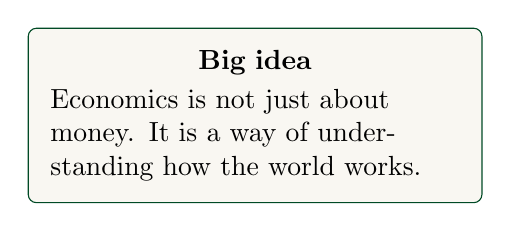
\begin{tikzpicture}
\node[draw=UNBCDark,rounded corners=3pt,fill=SoftCream,inner sep=8pt,text width=5.2cm] {
\centering\textbf{Big idea}\\[0.5ex]
Economics is not just about money. It is a way of understanding how the world works.
};
\end{tikzpicture}
\end{center}
\end{columns}
\end{frame}

\begin{frame}{What is economics?}
\topbanner{The simplest definition}
\vspace{0.2cm}
\begin{columns}[T,totalwidth=\textwidth]
\column{0.58\textwidth}
\begin{block}{Economics in plain language}
Economics is the study of how people, businesses, and governments make choices when resources are limited.
\end{block}
\vspace{0.1cm}
\begin{itemize}[<+->]
\item We all face scarcity: limited time, money, energy, and opportunities.
\item Because resources are limited, every choice has a trade-off.
\item Economics helps us think clearly about those trade-offs.
\end{itemize}

\column{0.38\textwidth}
\begin{mybox}{AccentOrange}
\centering
\textbf{Student example}\\[0.6ex]
Sleep\\
Good grades\\
Part-time job\\
Friends\\
Relaxation\\[0.6ex]
\textbf{Only 24 hours}
\end{mybox}
\vspace{0.15cm}
\centering\textcolor{UNBCDark}{\large That is economics.}
\end{columns}
\end{frame}

\begin{frame}{Economics is already part of everyday life}
\topbanner{You are already doing economics}
\vspace{0.15cm}
\begin{columns}[T,totalwidth=\textwidth]
\column{0.32\textwidth}
\begin{mybox}[height=4.7cm]{UNBCGreen}
\textbf{At home}\\[0.5ex]
\begin{itemize}
\item Grocery budgets
\item Saving vs. spending
\item Rent, mortgage, and bills
\item Family trade-offs
\end{itemize}
\end{mybox}

\column{0.32\textwidth}
\begin{mybox}[height=4.7cm]{AccentBlue}
\textbf{At school}\\[0.5ex]
\begin{itemize}
\item Choosing courses
\item Managing time
\item Working while studying
\item Planning the future
\end{itemize}
\end{mybox}

\column{0.32\textwidth}
\begin{mybox}[height=4.7cm]{AccentTeal}
\textbf{In society}\\[0.5ex]
\begin{itemize}
\item Inflation and wages
\item Housing affordability
\item Taxes and public services
\item Climate policy
\end{itemize}
\end{mybox}
\end{columns}
\vspace{0.25cm}
\centering\textit{Economics is what you are already doing - even if you never call it economics.}
\end{frame}

\begin{frame}{Four real-life examples}
\topbanner{Economics shows up in ordinary decisions}
\vspace{0.15cm}
\begin{columns}[T,totalwidth=\textwidth]
\column{0.48\textwidth}
\begin{mybox}{UNBCGold}
\textbf{Coffee shop line}\\
High demand + limited supply = waiting time.
\end{mybox}
\vspace{0.15cm}
\begin{mybox}{AccentRed}
\textbf{Concert tickets}\\
Scarce seats + huge demand = resale prices jump.
\end{mybox}
\vspace{0.15cm}
\begin{mybox}{AccentTeal}
\textbf{Grocery shopping}\\
Families switch products when prices rise.
\end{mybox}

\column{0.48\textwidth}
\begin{block}{Opportunity cost}
The real cost of a choice is the value of the next best alternative you give up.
\end{block}
\vspace{0.15cm}
\begin{mybox}{AccentBlue}
\textbf{Choosing a degree}\\
The question is not only \emph{What do I like?} but also \emph{What opportunities does it open?}
\end{mybox}
\vspace{0.2cm}
\textit{If you spend three hours scrolling instead of studying, economics politely asks: what did that really cost?}
\end{columns}
\end{frame}

\begin{frame}{The big questions economics helps explain}
\topbanner{From headlines to real life}
\vspace{0.1cm}
\begin{center}
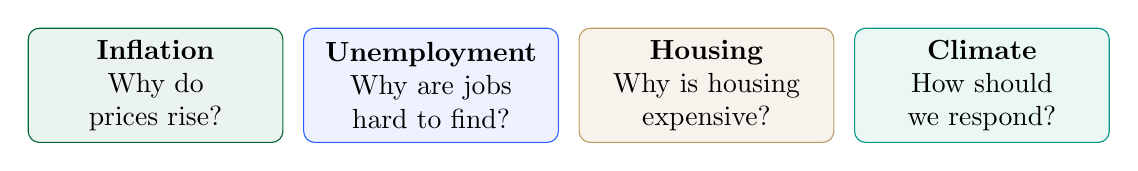
\begin{tikzpicture}[node distance=0.25cm]
\node[draw=UNBCGreen,fill=UNBCGreen!8,rounded corners=4pt,text width=3cm,minimum height=1.45cm,align=center] (a) {\textbf{Inflation}\\Why do prices rise?};
\node[draw=AccentBlue,fill=AccentBlue!8,rounded corners=4pt,text width=3cm,minimum height=1.45cm,align=center,right=of a] (b) {\textbf{Unemployment}\\Why are jobs hard to find?};
\node[draw=UNBCGold,fill=UNBCGold!12,rounded corners=4pt,text width=3cm,minimum height=1.45cm,align=center,right=of b] (c) {\textbf{Housing}\\Why is housing expensive?};
\node[draw=AccentTeal,fill=AccentTeal!8,rounded corners=4pt,text width=3cm,minimum height=1.45cm,align=center,right=of c] (d) {\textbf{Climate}\\How should we respond?};
\end{tikzpicture}
\end{center}
\vspace{0.35cm}
\begin{block}{A core economist habit}
Do not stop at the first effect. Ask: \textbf{what happens next?}
\end{block}
\vspace{0.1cm}
\begin{itemize}
\item Policies can help, but they can also create side effects and unintended consequences.
\item Economics trains us to look at the second and third round effects too.
\end{itemize}
\end{frame}

\begin{frame}{Economics is about people, not just numbers}
\topbanner{Human stories sit behind the statistics}
\vspace{0.1cm}
\begin{columns}[T,totalwidth=\textwidth]
\column{0.55\textwidth}
\begin{itemize}[<+->]
\item Families deciding how to use limited income
\item Students choosing what to study and where to work
\item Workers searching for stable jobs and better wages
\item Governments deciding how to spend limited budgets
\item Communities trying to improve quality of life
\end{itemize}

\column{0.4\textwidth}
\begin{mybox}{UNBCGreen}
\textbf{Important point}\\[0.7ex]
Good economics is deeply human. It studies well-being, fairness, incentives, and the consequences of choices.
\end{mybox}
\end{columns}
\end{frame}

\begin{frame}{Behavioural economics}
\topbanner{What if humans are not perfect decision-makers?}
\vspace{0.05cm}
\begin{columns}[T,totalwidth=\textwidth]
\column{0.56\textwidth}
\begin{itemize}[<+->]
\item Traditional economics often starts with rational decision-makers.
\item Behavioural economics studies how people \textbf{actually} behave.
\item It looks at procrastination, habits, overconfidence, peer effects, and self-control problems.
\item It helps explain why people delay saving, overspend, or stick with defaults.
\end{itemize}

\column{0.4\textwidth}
\begin{mybox}{AccentOrange}
\textbf{Everyday version}\\[0.6ex]
``Starting tomorrow, I will save more, exercise more, and stop buying things online.''
\end{mybox}
\vspace{0.15cm}
\begin{mybox}{AccentBlue}
\textbf{Funny truth}\\[0.6ex]
Humans are not robots. Sometimes we are not even very good spreadsheets.
\end{mybox}
\end{columns}
\end{frame}

\begin{frame}{Neuroeconomics}
\topbanner{Where economics meets psychology and the brain}
\vspace{0.15cm}
\begin{columns}[T,totalwidth=\textwidth]
\column{0.54\textwidth}
\begin{block}{What it studies}
Neuroeconomics examines what happens in the brain when people make choices involving risk, reward, trust, impulse, and emotion.
\end{block}
\vspace{0.1cm}
\begin{itemize}
\item Why do people take risks?
\item Why does immediate reward often beat long-term benefit?
\item How do emotions affect financial decisions?
\end{itemize}

\column{0.42\textwidth}
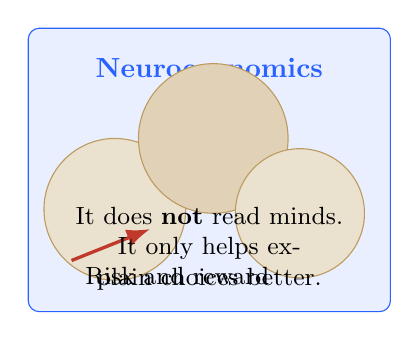
\begin{tikzpicture}[x=1cm,y=1cm]
\draw[fill=AccentBlue!10,draw=AccentBlue,rounded corners=4pt] (0,0) rectangle (4.6,3.6);
\node[font=\bfseries,text=AccentBlue] at (2.3,3.1) {Neuroeconomics};
\draw[fill=UNBCGold!30,draw=UNBCGold] (1.1,1.3) circle (0.9);
\draw[fill=UNBCGold!45,draw=UNBCGold] (2.35,2.2) circle (0.95);
\draw[fill=UNBCGold!30,draw=UNBCGold] (3.45,1.25) circle (0.82);
\draw[very thick,AccentRed,-{Latex[length=3mm]}] (0.55,0.65) -- (1.55,1.05);
\node[anchor=west,font=\small] at (0.6,0.45) {Risk and reward};
\node[align=center,text width=4.1cm,font=\small] at (2.3,0.8) {It does \textbf{not} read minds.\\It only helps explain choices better.};
\end{tikzpicture}
\end{columns}
\end{frame}

\begin{frame}{Other fascinating fields in economics}
\topbanner{Economics is broad, modern, and interdisciplinary}
\vspace{0.05cm}
\begin{multicols}{2}
\begin{mybox}{UNBCGreen}
\textbf{Labour economics}\\Jobs, wages, skills, unemployment.
\end{mybox}
\vspace{0.15cm}
\begin{mybox}{AccentTeal}
\textbf{Environmental economics}\\Climate, pollution, sustainability.
\end{mybox}
\vspace{0.15cm}
\begin{mybox}{AccentBlue}
\textbf{Health economics}\\Healthcare costs, access, and policy.
\end{mybox}
\columnbreak
\begin{mybox}{UNBCGold}
\textbf{Development economics}\\Poverty, education, growth, and living standards.
\end{mybox}
\vspace{0.15cm}
\begin{mybox}{AccentOrange}
\textbf{Financial economics}\\Banking, investing, markets, and risk.
\end{mybox}
\vspace{0.15cm}
\begin{mybox}{AccentRed}
\textbf{Public economics}\\Taxes, spending, and government policy.
\end{mybox}
\end{multicols}
\end{frame}

\begin{frame}{Why economics matters now more than ever}
\topbanner{A changing world needs economic thinking}
\vspace{0.1cm}
\begin{center}
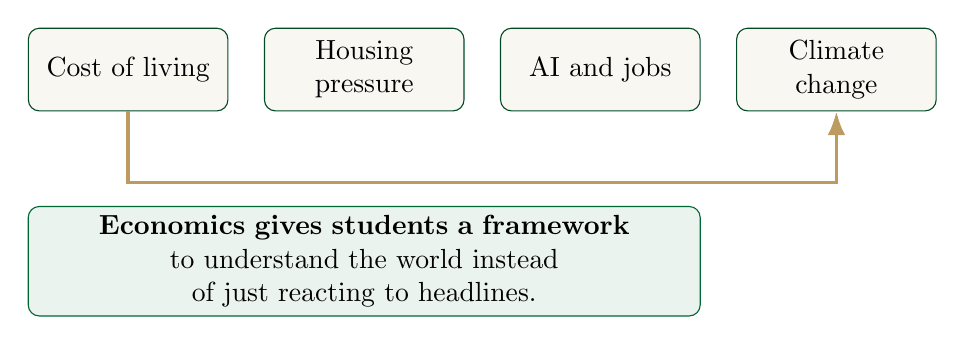
\begin{tikzpicture}[node distance=0.45cm]
\node[draw=UNBCDark,fill=SoftCream,rounded corners=4pt,text width=2.3cm,minimum height=1.05cm,align=center] (a) {Cost of living};
\node[draw=UNBCDark,fill=SoftCream,rounded corners=4pt,text width=2.3cm,minimum height=1.05cm,align=center,right=of a] (b) {Housing pressure};
\node[draw=UNBCDark,fill=SoftCream,rounded corners=4pt,text width=2.3cm,minimum height=1.05cm,align=center,right=of b] (c) {AI and jobs};
\node[draw=UNBCDark,fill=SoftCream,rounded corners=4pt,text width=2.3cm,minimum height=1.05cm,align=center,right=of c] (d) {Climate change};
\draw[very thick,UNBCGold,-{Latex[length=3mm]}] (a.south) -- +(0,-0.9) -| ($(d.south)+(0,-0.9)$) -- (d.south);
\node[below=1.2cm of b,draw=UNBCGreen,fill=UNBCGreen!8,rounded corners=4pt,text width=8.3cm,minimum height=1.25cm,align=center] (e) {\textbf{Economics gives students a framework}\\to understand the world instead of just reacting to headlines.};
\end{tikzpicture}
\end{center}
\end{frame}

\begin{frame}{What skills does economics build?}
\topbanner{Skills for university, work, and life}
\vspace{0.05cm}
\begin{columns}[T,totalwidth=\textwidth]
\column{0.48\textwidth}
\begin{mybox}{UNBCGreen}
\textbf{Analytical skills}
\begin{itemize}
\item Critical thinking
\item Problem solving
\item Data interpretation
\item Decision-making under uncertainty
\end{itemize}
\end{mybox}

\column{0.48\textwidth}
\begin{mybox}{AccentBlue}
\textbf{Transferable skills}
\begin{itemize}
\item Clear writing and communication
\item Understanding incentives
\item Spotting unintended consequences
\item Connecting evidence to policy
\end{itemize}
\end{mybox}
\end{columns}
\vspace{0.25cm}
\centering\textit{These are not only economist skills. They are career skills and life skills.}
\end{frame}

\begin{frame}{Why students should consider economics}
\topbanner{Practical, flexible, and career-relevant}
\vspace{0.1cm}
\begin{columns}[T,totalwidth=\textwidth]
\column{0.52\textwidth}
\begin{itemize}[<+->]
\item Economics is practical and relevant to everyday life.
\item It combines numbers, ideas, and real-world problems.
\item It works well on its own or with business, political science, data science, and environmental studies.
\item It opens doors to many careers.
\end{itemize}

\column{0.43\textwidth}
\begin{mybox}{UNBCGold}
\textbf{Common pathways}
\begin{itemize}
\item Government and public policy
\item Banking and finance
\item Business and consulting
\item Research and analytics
\item Law, education, and graduate study
\end{itemize}
\end{mybox}
\end{columns}
\end{frame}

\begin{frame}{A message for students and parents}
\topbanner{Why economics is worth serious consideration}
\vspace{0.15cm}
\begin{columns}[T,totalwidth=\textwidth]
\column{0.48\textwidth}
\begin{mybox}{UNBCGreen}
\textbf{For students}\\[0.6ex]
If you are curious about how the world works and enjoy asking ``why,'' economics is worth exploring.
\end{mybox}
\vspace{0.25cm}
\begin{mybox}{AccentBlue}
\textbf{For parents}\\[0.6ex]
Economics develops adaptable, analytical, employable graduates with skills valued across many sectors.
\end{mybox}

\column{0.46\textwidth}
\begin{block}{A light joke}
After one economics course, students may finally understand why ``we cannot buy everything'' is not just parenting. It is scarcity.
\end{block}
\vspace{0.2cm}
\begin{mybox}{UNBCGold}
\textbf{Bottom line}\\[0.6ex]
Economics helps people make better choices, ask better questions, and understand the world more clearly.
\end{mybox}
\end{columns}
\end{frame}

\begin{frame}[plain]
\usebackgroundtemplate{\includegraphics[width=\paperwidth,height=\paperheight]{/mnt/data/user-fE7TD4iShS4hrCs2AD7Tw51y/5c309b8515dc4e28a392dd530e83cc2b/mnt/data/econ_montage.png}}
\begin{tikzpicture}[remember picture,overlay]
\fill[UNBCDark,opacity=0.83] (current page.south west) rectangle (current page.north east);
\node[text=white,font=\bfseries\fontsize{24}{28}\selectfont,align=center] at (current page.center) {Economics is not just a subject.\\[0.2cm]It is a way of understanding the world.};
\node[text=UNBCGold,font=\Large,align=center] at ([yshift=-1.6cm]current page.center) {Thank you};
\node[text=white,font=\normalsize,align=center] at ([yshift=-2.25cm]current page.center) {Questions?};
\end{tikzpicture}
\end{frame}

\end{document}
